\chapter{Fundamentals of the Riemann Pump}
\label{ch:fundamentals}
%\textit{Presentation of the theoretical basis required for an understanding of your work. Do not begin with Newton's laws or Maxwell's equations: imagine that the reader is a competent engineering professor, but not necessarily in your field of expertise. Do not bother to discuss any theory that you do not employ in later sections.}
To place this work into the context of the next generation of mobile communication, a concept is described called software-defined radio.
Implemented in this concept, the function, the benefit and some fundamentals of the Riemann Pump are described. 
A demonstrated system shows the \gls{ab:sdr} concept, which is based on the idea to bring the digital domain as close as possible to the antenna.
The Riemann Pump is an arbitrary waveform generator which is controlled by a digital input signal, making it also a custom \gls{ab:dac}.
The concept of the custom designed \gls{ab:dac} as well as some characteristics are presented.
A concise discussion conclude the presented fundamentals.

% Because the analog output signal should be transmitted via an antenna, it has to be enough output power.
%The number of bits, hence the resolution of the \gls{ab:dac} is less stringent as the digital to analog conversion do not distinguish so much within the digital code.
% A crucial point to increase the performance is the oversampling ratio. 
% As the analog signal could consist with some concurrent signals, linearity is crucial to avoid unwanted distortions.
%All these requirements built in one \gls{ab:dac} is not realistic.
%Therefore, intermediate systems have been developed in which the transmitter signal is built by a DAC at lower frequencies, and then up converted with RFFE mostly composed by a linear mixer with a linear PA.
\section{Basic concept of software-defined radio for 5G mobile communication}
The concept of software-defined radio is treated to overcome old problems of mobile communication and hence deal with a fast adapting system which can handle several mobile communication standards at once. % which problems? either state it or leave it
New standards can handled since the system can be changed with an firmware update. 
Therefore every signal within the proposed bandwidth could be processed without changing the hardware, which made it software defined.
The ability to process a spectrum of \gls{ab:dc} to \SI{6}{\giga \hertz} enables it to deal with future mobile communication standards.\\
%, e.g. IEEE802.11ac (\gls{ab:wlan}) and \gls{ab:lte} already work at \SI{5}{\giga \hertz} and \SI{0.7} ... \SI{2.6}{\giga \hertz}, respectively.\\
To achieve this goal it is essential to bring the digital domain as close as possible to the antenna \cite{RivetDevalBegueretJ.-B.2007}, \cite{DevalRivetVeyracEtAl2013},\cite{RivetDevalJ.-B.EtAl2010}.
The digital domain has a lot of advantages regarding complexity, cost, filtering and processing speed \cite{Grossman2005}, \cite{Maroldt2010}.
The structure of digital components is less complex and therefore has less cost.
Digital filtering is more precise and data processing is more efficient and faster \cite{Chamberlain2015}, \cite{LiRaghunathanJha2009}.\\
The ultimate software defined radio architecture is shown in Figure \ref{fig:ultimateSDR}.

\begin{figure}[ht]
	\centering
  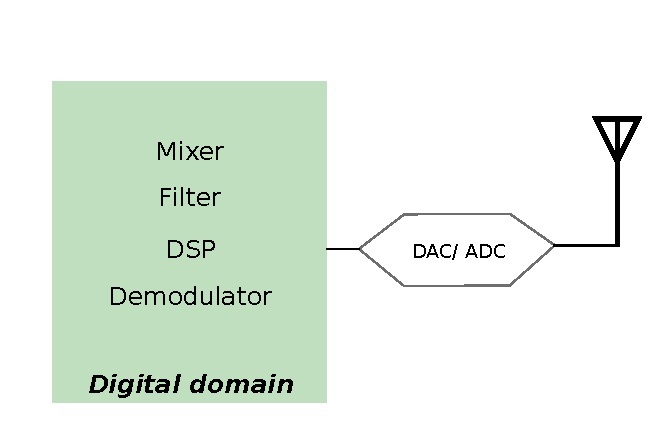
\includegraphics[width=.5\textwidth]{ultimateSDR.pdf}
	\caption{Ultimate Software-defined radio architecture \cite{DevalRivetVeyracEtAl2013}}
	\label{fig:ultimateSDR}
\end{figure}

In this vision the analog received signal is directly converted into the digital domain and afterwards filtered, mixed, demodulated and processed.
For the transmission path the process is vice versa.
The absence of the \gls{ab:rffe} is a dream still to come true \cite{RivetDevalJ.-B.EtAl2010}.\\
Figure \ref{fig:feas_energy} shows the feasibility (left) and the estimated power consumption (right) evaluated in \cite{RivetDevalJ.-B.EtAl2010}.
The illustration shows that this vision is not a realistic option yet.

\begin{figure}[htbp]
	% minipage mit (Blind-)Text
	\begin{minipage}{0.49\linewidth} 
	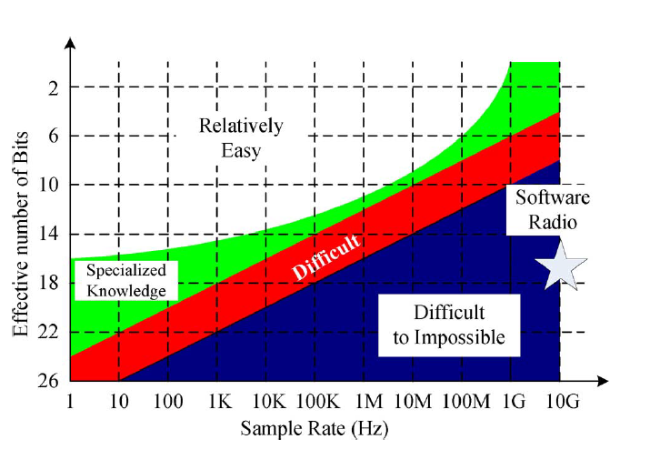
\includegraphics[width=1.1\textwidth]{energy_consumption_sdr.pdf}
	%\caption{Feasibility of Software Radio}
	%\label{energy1} 
	\end{minipage}
	% Auffüllen des Zwischenraums
	\hfill
	% minipage mit Grafik
	\begin{minipage}{0.49\linewidth}
	% \textwidth bezieht sich nun auf die Minipage
	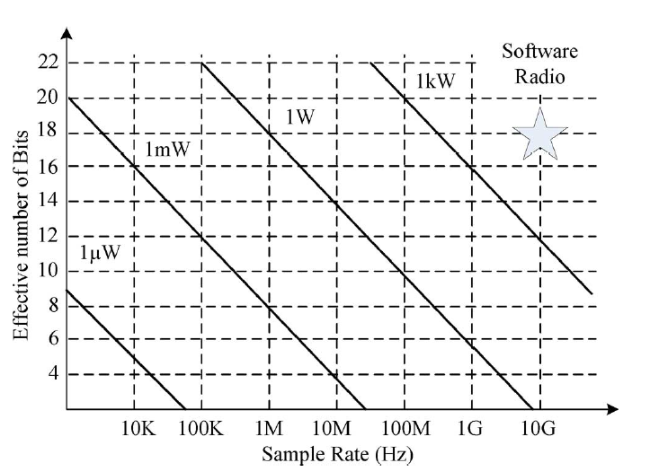
\includegraphics[width=1.1\textwidth]{energy_consumption_sdr2.pdf}
	%\caption{Estimated energy consumption}
	%\label{energy2} 
	\end{minipage}
 \caption{Feasibility (left) and estimation of energy consumption (right) regarding Effective number of Bits and Sample Rate \cite{RivetDevalJ.-B.EtAl2010}}
 \label{fig:feas_energy}
\end{figure}

To reach modern \gls{ab:rf} standards a \gls{ab:enob} of 17 is required while ensuring a sample rate of \SI{10}{\giga \hertz} to process baseband signals in the \si{\giga \hertz} range.
As shown in in Figure \ref{fig:feas_energy} on the left side, the development of an \gls{ab:adc} or \gls{ab:dac} with modern technologies is difficult to impossible with respect of the mentioned requirements.
Another critical bottleneck in this concept is the power consumption, shown on the right side.
A power consumption in the range of \si{\kilo \watt} occurs if the requirements for modern \gls{ab:rf} standards are fulfilled.
This identification of drawbacks makes the analog \gls{ab:rffe} indispensable.
The pre-processing of the analog signal in the receiving path is required to reduce the energy consumption to a moderate range.
While for the transmitting path, the concept of the Riemann Pump comes into play.

\section{System design using the Riemann Pump} % PLL and Energy consumption
The focus in this thesis was on the transmitting path of the mentioned system, since the receiving architecture and concepts need a separate investigation.
Further details on the receiving concepts and investigations can be found in  \cite{RivetDevalBegueretJ.-B.2007}, \cite{RivetFadhuileDevalEtAl2013}, \cite{RivetDevalD.2008}, \cite{RivetF.2014}.
Since the transmitting path is considered, the need for a \gls{ab:dac} becomes visible, as the digital data must be converted to an analog signal before transmission.
As mentioned before high demands are made to the \gls{ab:dac} implemented in a \gls{ab:sdr} concept.\\
An important requirement is to keep the energy consumption in a moderate range.
If the consumed energy is in the range of several \si{\kilo \watt} (Figure \ref{fig:feas_energy}) it is clear that this is unworkable.
In order to meet \gls{ab:rf} standards the \gls{ab:snr} has to fulfil the given limits. %which limits?
To achieve a moderate \gls{ab:snr}, the resolution and the \gls{ab:osr} of the \gls{ab:dac} have to meet the requirements.
The generated analog output signal, which can consist of a few concurrent signals, has to be amplified for the propagation.
To avoid unwanted distortions in the propagated signals linearity of the system is crucial.\\
% Therefore there is no intermediate step of signal processing which decrease the latency.
%The benefit of this concept is to realize this \gls{ab:dac} as close as possible to the RF front end without an intermediate step of analog signal processing.
% The main drawback of this approach is the energy consumption based on an inefficient ADC/DAC.
%Based on this concept a digital-analog converter is designed to deal with a higher bandwidth than other devices nowadays.
Figure \ref{fig:System} demonstrates the transmitting path of the system design for the concept of \gls{ab:sdr} with the implementation of the Riemann Pump.

\begin{figure}[ht]
	\centering
  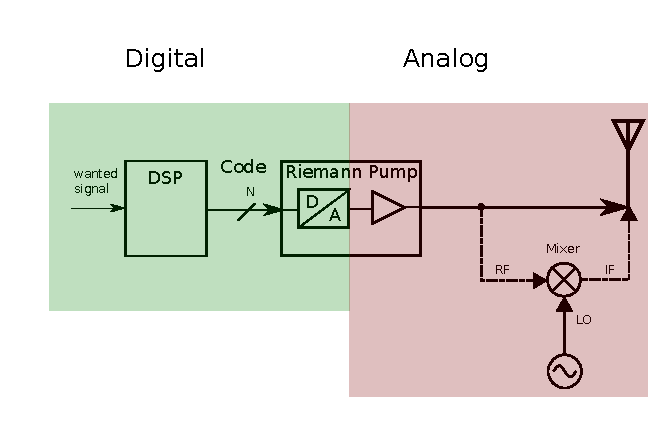
\includegraphics[width=\textwidth]{SystemDesign.pdf}
	\caption{Concept of the Software-defined radio}
	\label{fig:System}
\end{figure}

The demonstrated path in Figure \ref{fig:System} is subdivided into a digital and analog part.
The green digital part is responsible for the calculation of the desired signals and the generation of the corresponding digital code.
A theoretical wanted signal in the time domain, consisting of multiple modulated signals, is fed to a \gls{ab:dsp} which computes a digital bit-stream.
The so called Riemann Code controls the input of a custom \gls{ab:dac}, called Riemann Pump, which is the interface between the digital and the analog part.\\
In the red analog domain the desired signal is amplified by an implemented power transistor in the Riemann Pump and then propagated via the antenna.
Optionally a mixer can be connected to mix the desired signal to even higher frequencies of several tenth of \si{\giga \hertz}.\\
Beside the advantages of the concept there are some constraints on the energy consumption as well as on the real time emission.
Energy consumption is increasing linear with the switching frequency and therefore with the signal bandwidth.
Secondly the real time emission is constrained due to the calculation and conversion of the Riemann Code.

\section{Idea of the Riemann Pump}
\label{IdeaRiemannPump}
After the implementation in a system design has been demonstrated, the concept of Riemann Pump itself is explained.\\
The concept shown in Figure \ref{fig:ChargePump}, is implemented in conventional \glspl{ab:pll} and is known as a charge pump, which is the basic principle of the Riemann Pump \cite{DevalRivetVeyracEtAl2013}, \cite{VeyracRivetDevalEtAl2014}, \cite{DevalRivetVeyrac2015}.
Basically the inputs are switches and the output is a capacitance.
The output capacitance (\gls{sy:Cout}) can take any value between the positive (\gls{sy:Vdd}) and negative (\gls{sy:Vss}) power supply voltage by controlling the input switches.\\
 %  A PLL charge pump is merely a bipolar switched current source. This means that it can output positive and negative current pulses into the loop filter of the PLL. It cannot produce higher or lower voltages than its power and ground supply levels.
 The integration of the electrical current (\gls{sy:iout}) at the capacitance (\gls{sy:Cout}), to form the output voltage  (\gls{sy:Vout}), recalls the founder of the integration principle, Bernhard Riemann.
This integration and the concept of the charge pump lead to the name Riemann Pump, first mentioned in 2013 \cite{DevalRivetVeyracEtAl2013}. \\
Figure \ref{fig:ChargePump} shows the basic principle of a charge pump, used for the digital to analog conversion in this thesis.

% microsoft visio created charge pump
%\begin{figure}[ht]
%	\centering
%  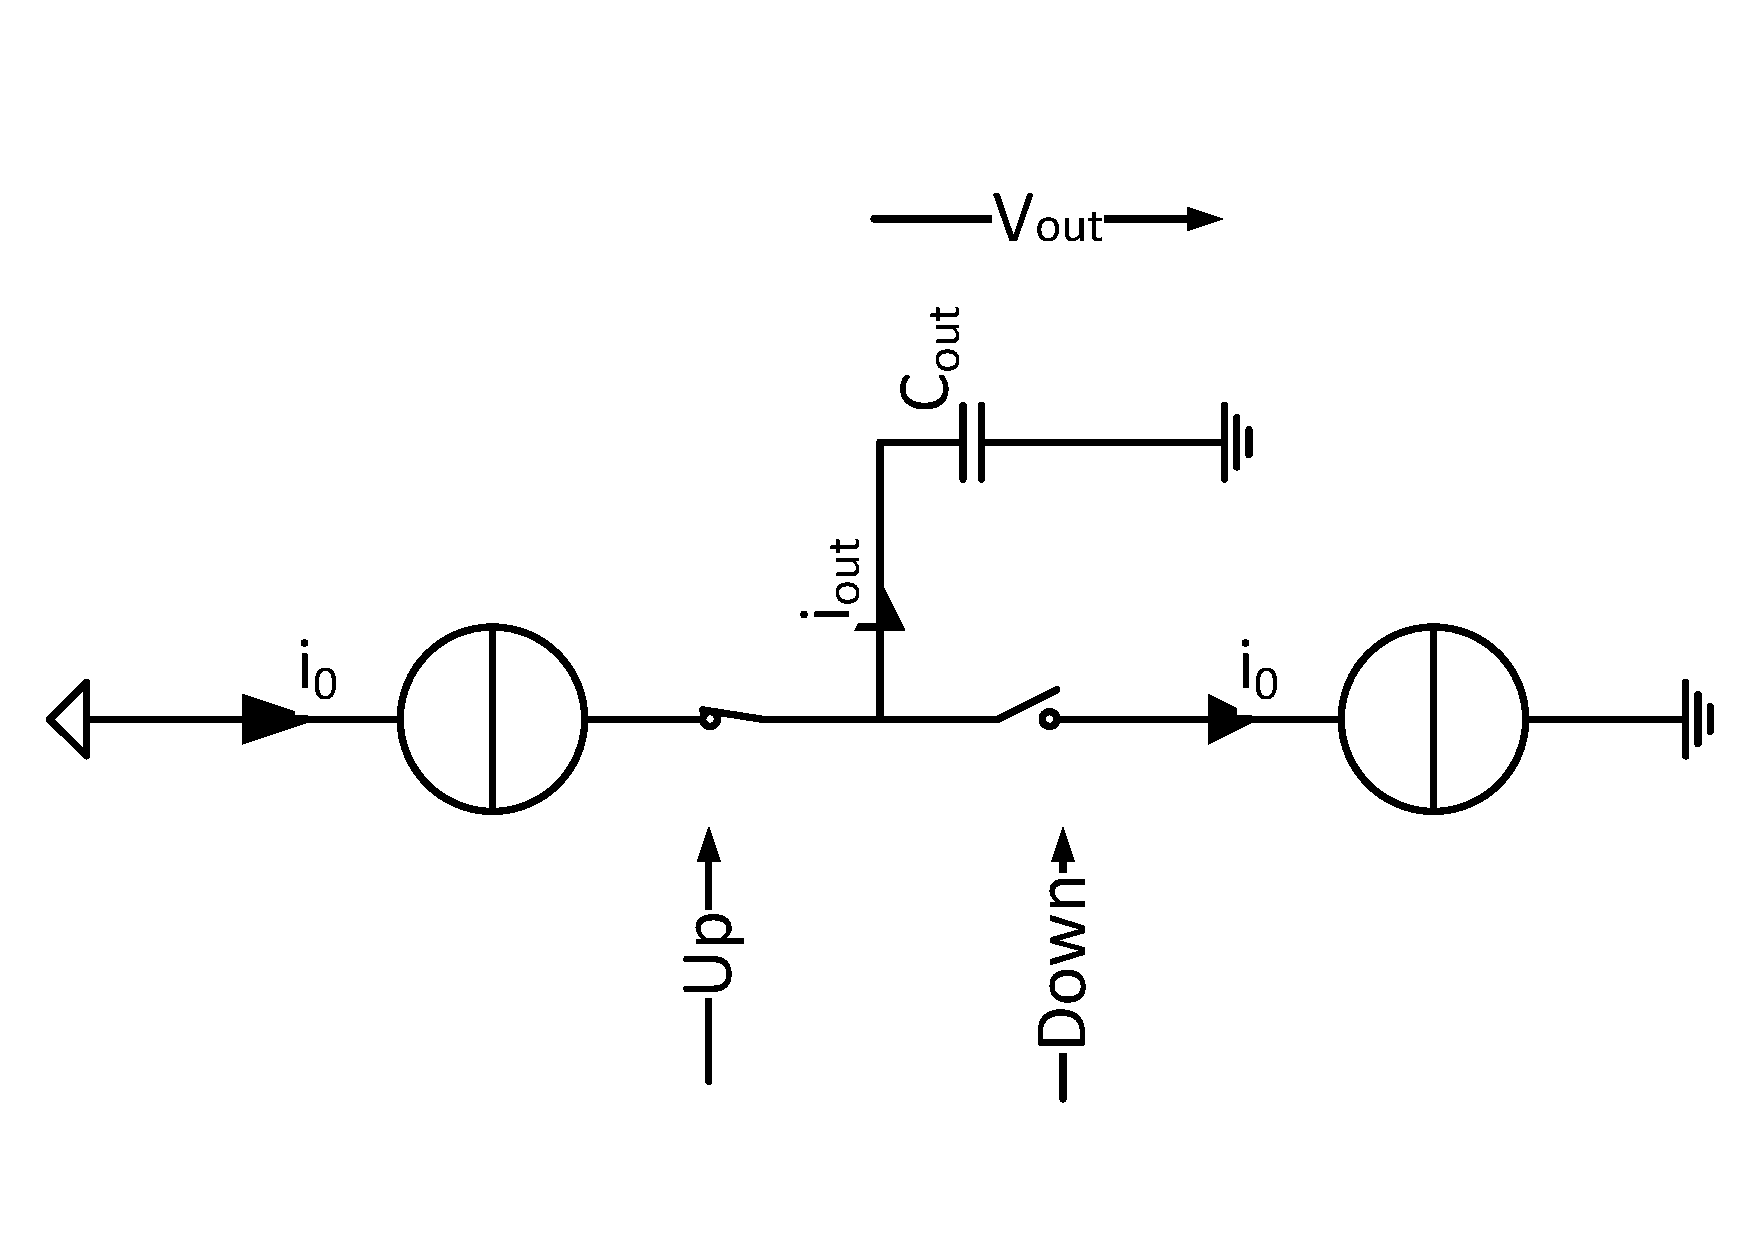
\includegraphics[width=0.5\textwidth, angle = 270]{ChargePump.pdf}
%	\caption{scheme of a charge pump}
%	\label{fig:ChargePump}
%\end{figure}

% inkscape created charge pump
\begin{figure}[ht]
	\centering
  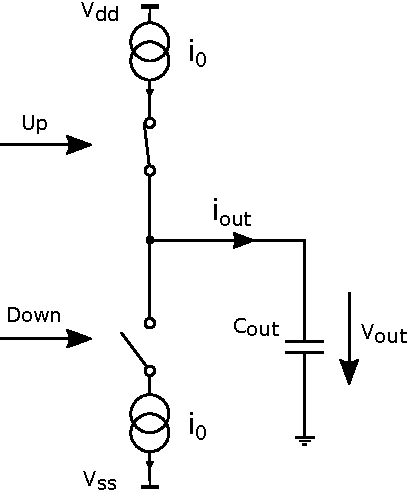
\includegraphics{ChargePump_ink.pdf}
	\caption{scheme of a charge pump}
	\label{fig:ChargePump}
\end{figure}

Two switches are shown, which are capable to switch current to and from the output capacitance, respectively.
The high side switch, which pushes charges onto the output capacitance, is connected to a current source at \gls{sy:Vdd}.
In contrast to that, the low side switch is connected to a current source at \gls{sy:Vss}.
While controlling the switches with a differential input signal, the output voltage can be varied between \gls{sy:Vdd} and \gls{sy:Vss}.
As the control signal only consists of closing and opening a switch, a digital signal is sufficient.
If the high side switch is closed while the low side switch is opened, charges are pumped to the capacitance which leads to an increase in output voltage.
This effect only takes place if the control signal is differential, which leads to synchronous switching behaviour of both switches.
Otherwise the controlling of the output voltage is not defined.
If both switches are closed at the same time, the potential at the capacitor is floating and hence no defined voltage can be stated.
For decreasing the output voltage the low side switch has to be closed, while the high side switch is open, to allow the capacitor to discharge.\\
Corresponding to the described principle, the output voltage
\begin{equation}
	V_{out} = \frac{1}{C_{out}}{ \int_0^T \! i_{out}(t) \, \mathrm{d}t}
\end{equation} %%, \hspace{1cm} T = \frac{2*OSR}{f_{sample}
 is calculated by integrating the current over time.\\
A custom \gls{ab:dac} is created by extending the basic charge pump with several other charge pumps in parallel, as seen in Figure \ref{fig:RiemannPumpConcept}.
Since the output voltage, consisting of the desired signals, should be propagated via an antenna, the output capacitance \gls{sy:Cout} can be interpreted as the input stage of a linear power amplifier. 
This input stage consists of a power transistor, which do have the capacitive input impedance characteristic.
Implemented in one component this concept saves area and costs and the amplified signal at the drain can be transmitted via the antenna.

\begin{figure}[H]
	\centering
  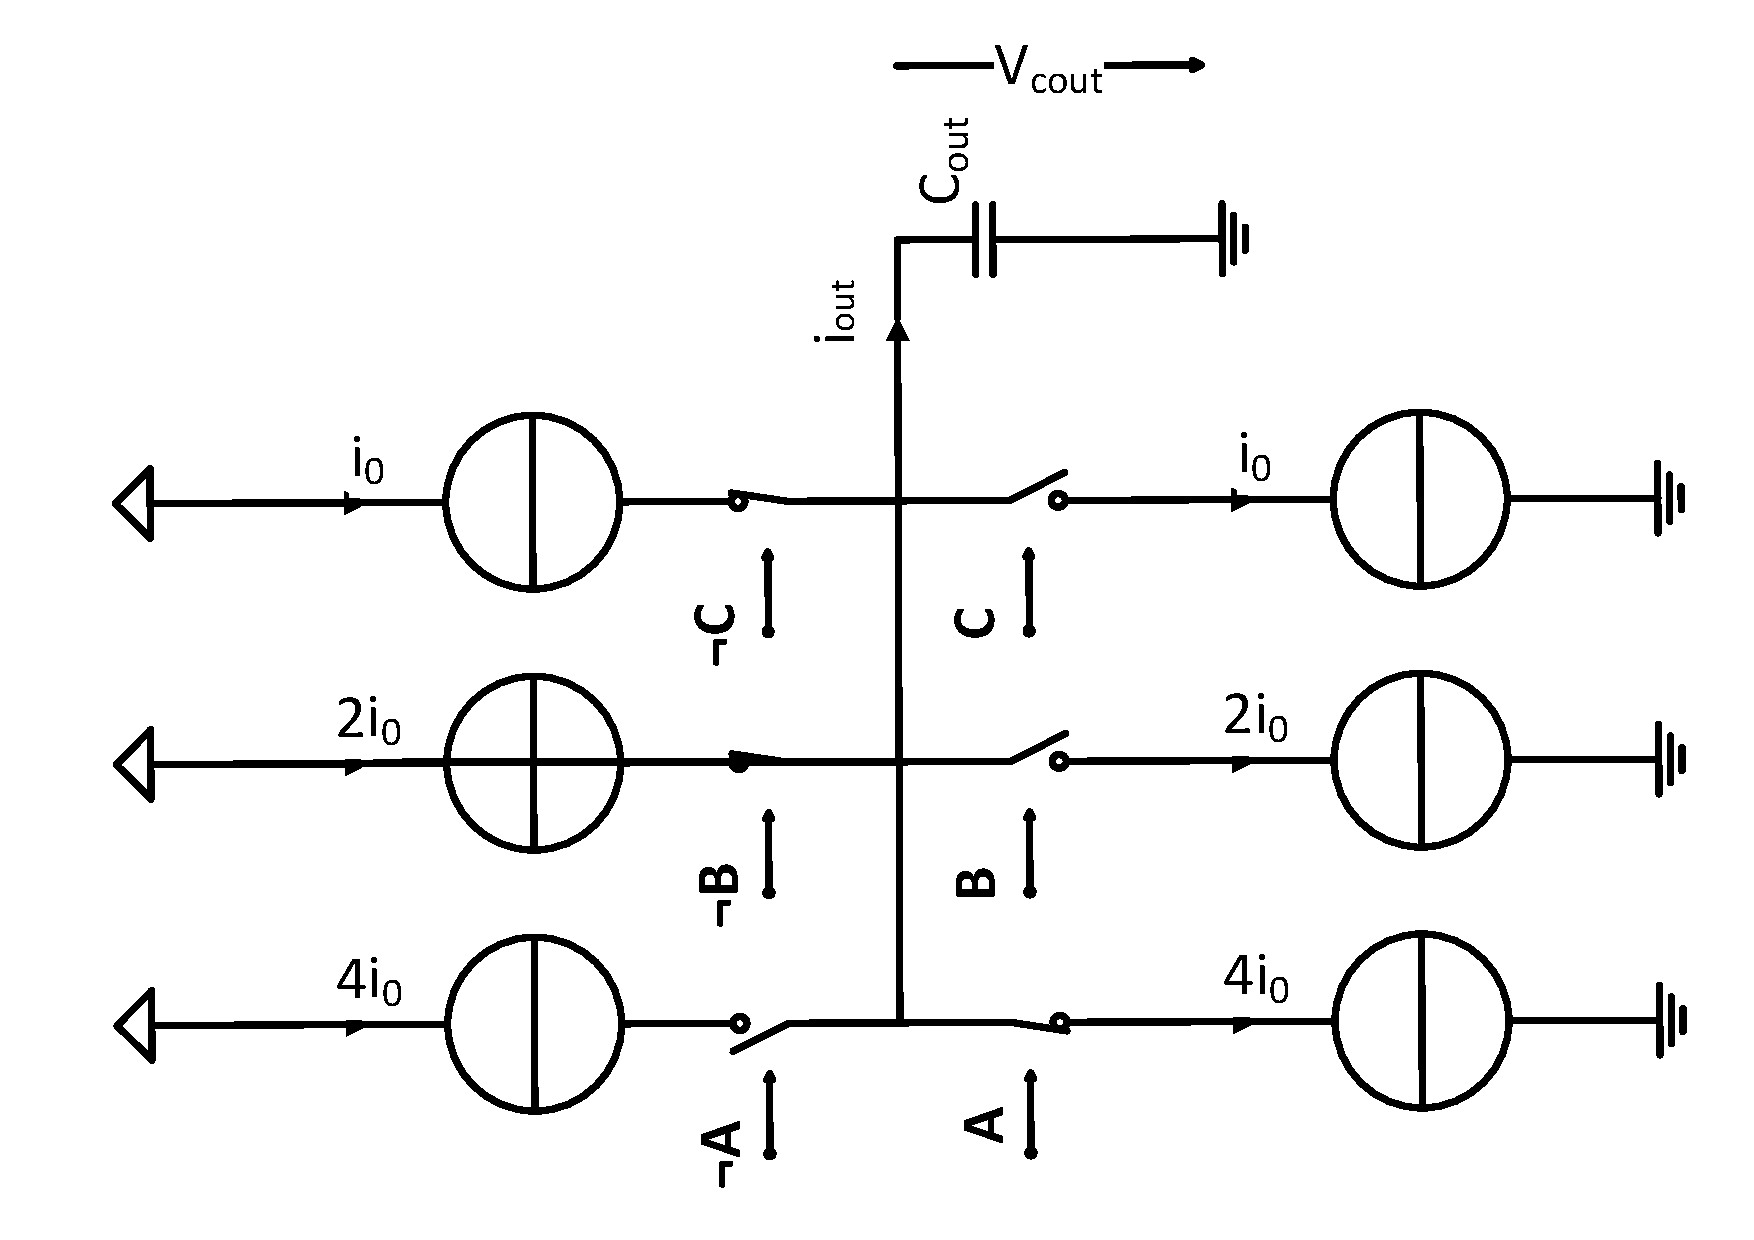
\includegraphics[scale=.4, angle = 270]{RP_concept.pdf}
	\caption{Concept of the Riemann Pump with three-bit resolution}
	\label{fig:RiemannPumpConcept}
\end{figure}

The dimensions of the current sources, connected in parallel, have to increase by the power of two to get a defined set of currents.
Otherwise two states would share the same code which will lead to a loss of information.
Demonstrated is a \gls{ab:dac} with three bit resolution, which leads to eight different output currents.
Instead of using absolute current values, relative currents with respect to $i_0$ are used.

\newpage
\section{Riemann Code generation}
The three bit resolution leads to eight different slopes which are presented in Figure \ref{fig:SlopesAndTable}.

\begin{figure}[H]
	\centering
  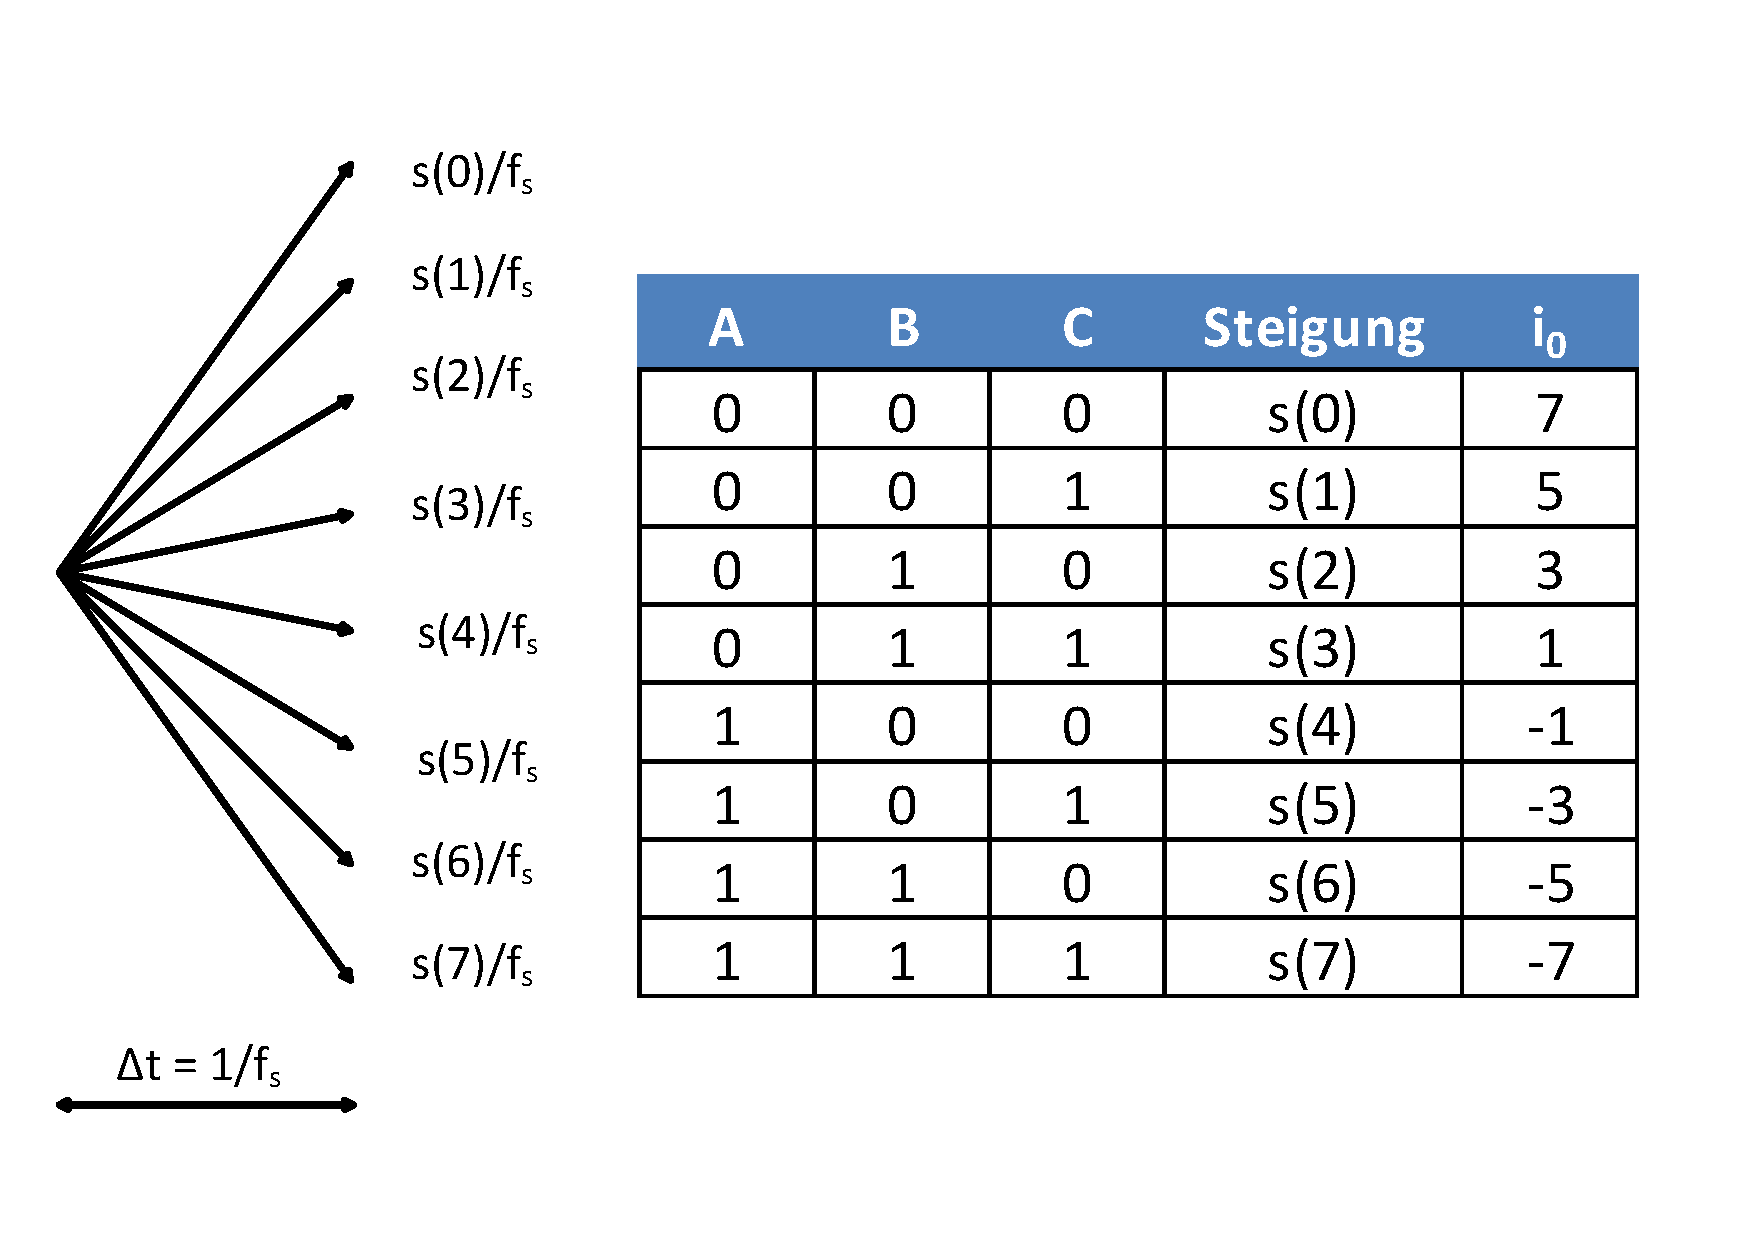
\includegraphics[width=\textwidth]{SlopesAndTable.pdf}
	\caption{slopes and corresponding code of the synthesized signal}
	\label{fig:SlopesAndTable}
\end{figure}

Corresponding to the demonstrated eight different slopes on the left side, a table is presented which states the corresponding encryption for each slope on the right side.
For example the representation of the relative slope of $-1 i_0$ is: $1 0 0 \equiv s(4)$.
Each digit of the code states the position of the corresponding switches (A, B and C), that is 0 for opened and 1 for an closed switch.
Figure \ref{fig:CodeGenerationPrinciple} shows the principle of the generation process.
% Code generation

 \begin{figure}[H]
	\centering
  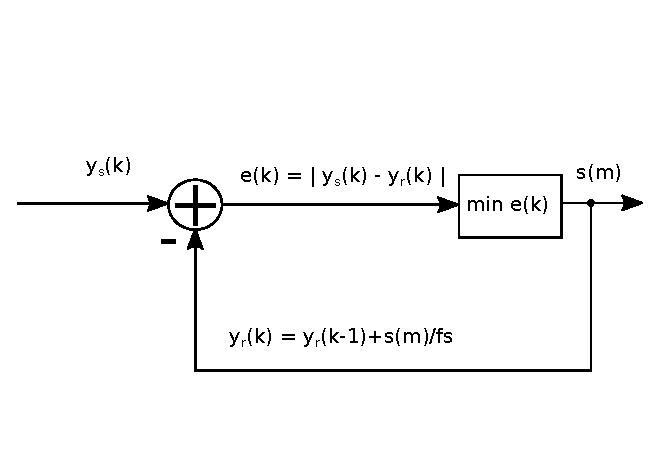
\includegraphics{CodeGenerationPrinciple.pdf}
	\caption{Code generation principle}
	\label{fig:CodeGenerationPrinciple}
\end{figure}

This principle states that a sampled version of the desired signal exists ($y_s$) which is subtracted by a linear approximated signal $y_r$ to obtain the error which then is minimized.
For every sampling point k, the relative slope $s(m)$ (m belonging to $[0,2^N-1]$; N number of bits) is chosen which minimizes the error 
\begin{equation}
e(k) = | y_s(k) - y_r(k) |.
\label{eq:error}
\end{equation}

The estimated value of $y_r(k)$ is represented by the sum of its previous value and the chosen slope times the sampling interval ($\frac{1}{f_{sampling}}$) yielding:
\begin{equation}
	y_r(k) = y_r(k-1) + \frac{s(m)}{f_{sampling}}.
	\label{eq:linearapproxsignal}
\end{equation}

The estimated signal $y_r$ (Equation \ref{eq:linearapproxsignal}) thus presents the sampled signal and generates the corresponding Riemann Code.
The benefit of the closed loop principle is that the recovered signal after integration, do not drift.
In comparison to this, in an open loop principle the difference between the current $y_s(k)$ and the previous input sample $y_s(k-1)$ is quantified and thus lead to a cumulative error in the recovered signal \cite{VeyracRivetDevalEtAl2016}.
An illustration of the closed loop generation of the Riemann Code is shown in Figure \ref{fig:RiemannIntegralError}.

 \begin{figure}[H]
	\centering
  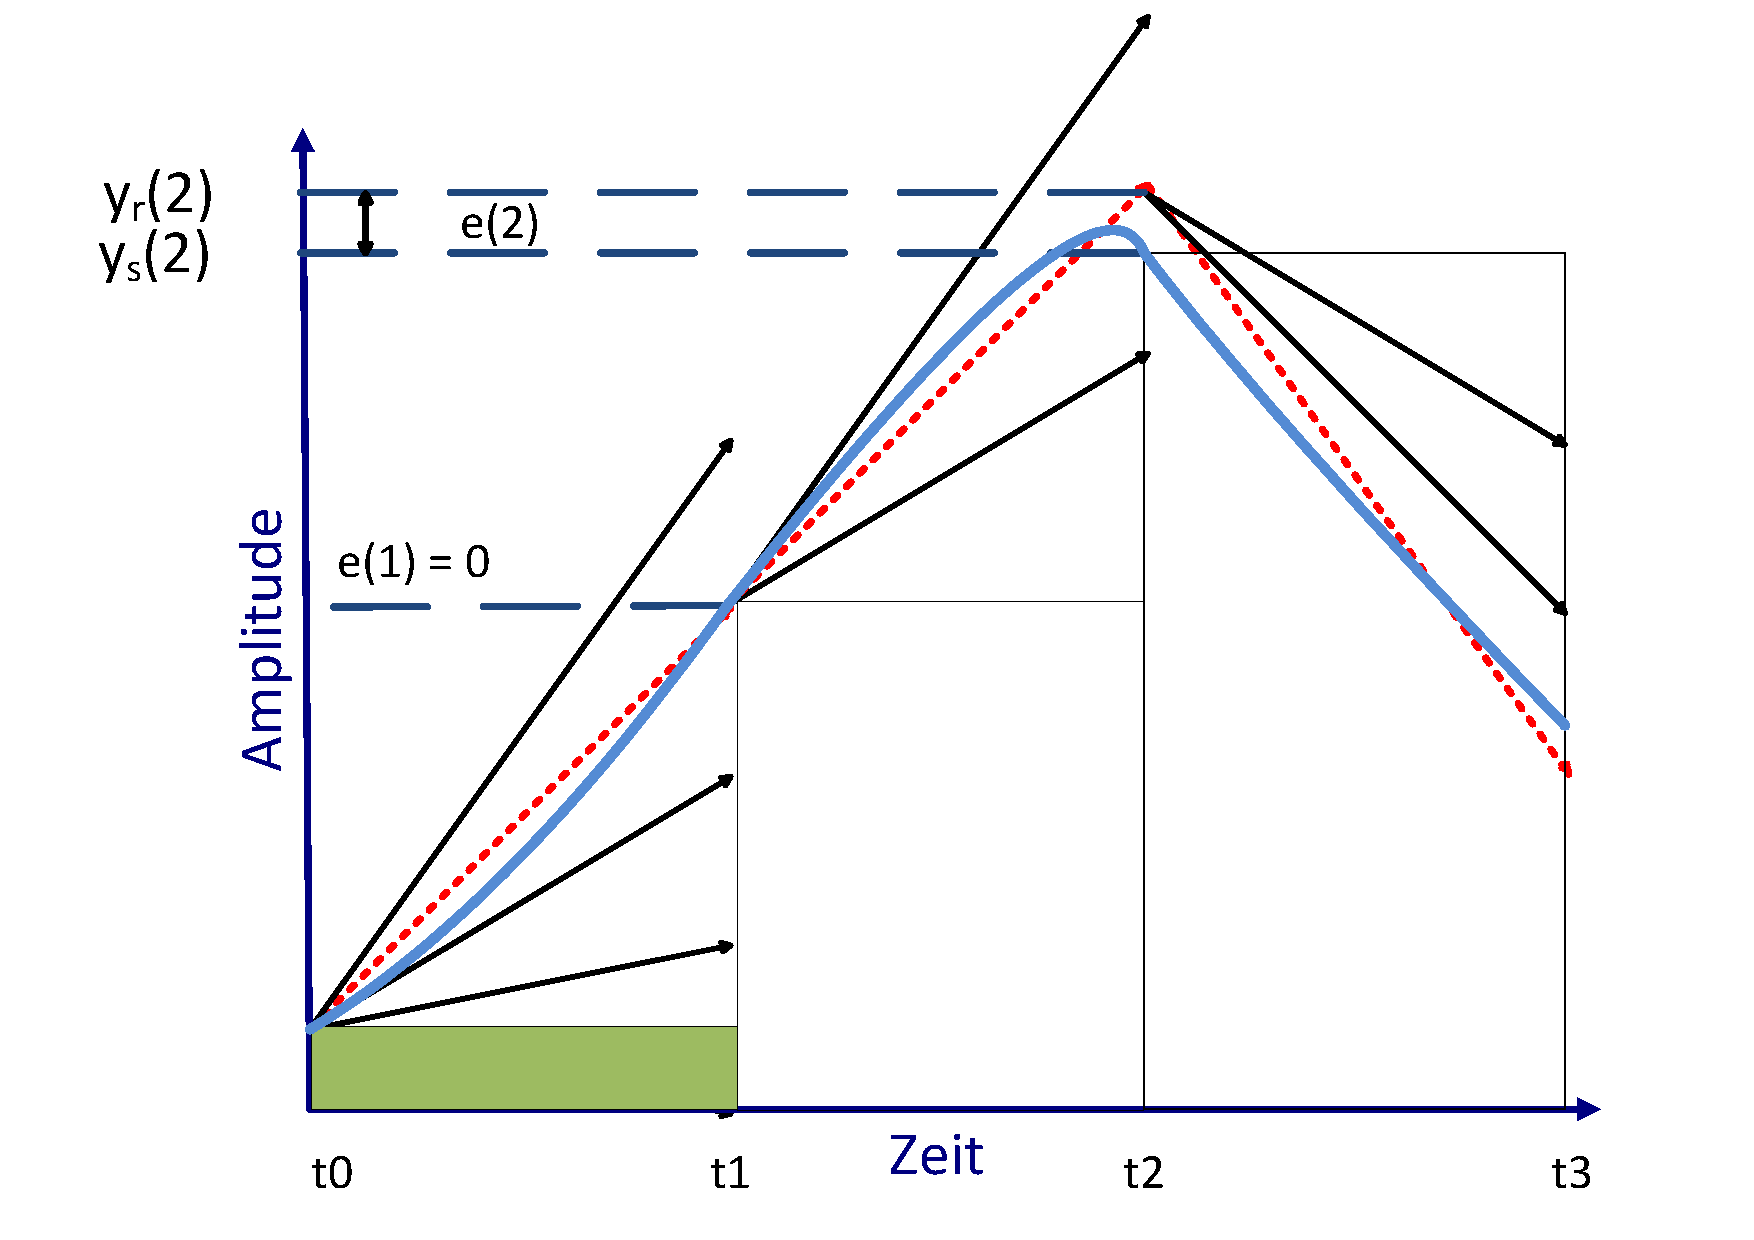
\includegraphics[width=\textwidth]{RiemannIntegralError.pdf}
	\caption{Code generation - error minimizing}
	\label{fig:RiemannIntegralError}
\end{figure}

The blue signal is the desired sampled input signal, the red is the linear approximation of the signal which generates the Riemann Code.
For the sampling point at time $t1$ no error exists since the linear approximation fit perfectly to the sampled input signal.
At the discrete time point $t2$ the slope $s(m)$ was chosen which minimized the error stated in Equation \ref{eq:error}.
The chosen slope is encrypted with the digital representation as shown in Figure \ref{fig:SlopesAndTable}.
This principle is used in an iterative way to generate a full sequence of slopes for the desired signal.
This sequence of slopes represents the Riemann Code for the desired signal.
Figure \ref{fig:RiemannIntegral} illustrates an example for generating a Riemann Code.

\begin{figure}[H]
	\centering
  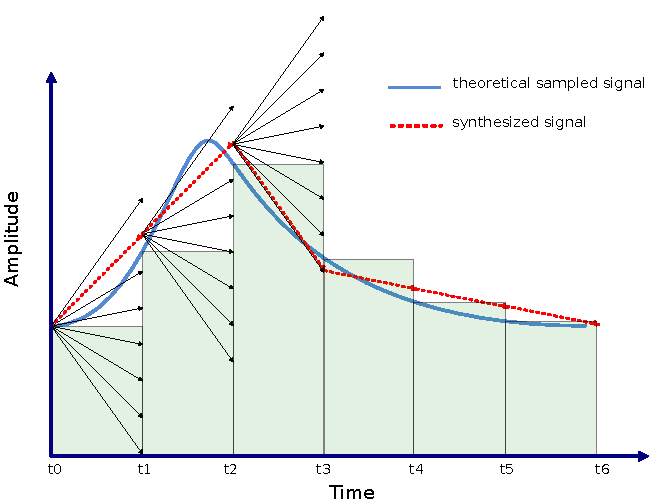
\includegraphics[width=\textwidth]{RiemannIntegral.pdf}
	\caption{Integral of the current which pumps charges on to the cap.}
	\label{fig:RiemannIntegral}
\end{figure}

In this example the sequence of slopes is
\begin{equation}
s(1)\hspace{.3cm} s(1)\hspace{.3cm} s(7)\hspace{.3cm} s(4)\hspace{.3cm} \equiv \hspace{.3cm} +5i_0\hspace{.3cm} +5i_0\hspace{.3cm} -7i_0\hspace{.3cm} -1 i_0,
 \end{equation} 
 for the time interval $[t0,t4]$ which generates the Riemann Code:
\begin{equation}
001\hspace{.3cm} 001\hspace{.3cm} 111\hspace{.3cm} 100\hspace{.3cm}.
\label{eq:RiemannCodeSineWave} 
\end{equation}

The desired signal, consisting of multiple different signals where each can have a different modulation and symbol rate, is pre processed and then sampled with the Riemann Conversion.
Using this technique arbitrary waveforms can be generated avoiding that the signal drift.

\section{Characteristics of Digital-to-Analog converter}
\label{ch:characteristics}
%The characteristics, the performance and figure of merits are compared to classify the Riemann Pump with the conventional digital-to-analog conversion principles.
%Performance: Resolution, Maximum sampling rate, dynamic range.
%FOM: Gain, SFDR, SNR, settling time.\\
%The characteristics of different \gls{ab:dac} is the performance and some figure of merits.
%Performance leads to the generation of noise in terms of signal to (quantization) noise ratio.
%This \gls{ab:sqnr} gave a good insight to the performance of the corresponding \gls{ab:dac} without to focus on energy consumption nor efficiency.\\ %%% 16:03 25.04.2016
To reach modern \gls{ab:rf} standards, a minimum amount of resolution and oversampling is needed.
Oversampling is crucial for the recovery of a signal, due to the Nyquist-Shannon sampling theorem
\begin{equation}
f_{Nyquist} = 2 f_{signal,max}.
\end{equation}
\label{eq:SamplingTheorem}

This Nyquist Frequency is the minimum sampling frequency for the correct recovery of a signal.
That means the actual sampling rate \gls{sy:fsampling} has to be at least two times \gls{sy:fsignalmax}.\\
Every increase of \gls{sy:fsampling} above the \gls{sy:fnyquist} is called oversampling.
To increase the performance of the \gls{ab:dac} an \gls{ab:osr} is introduced \cite{DevalRivetVeyrac2015}:
\begin{equation}
OSR = \frac{f_{sampling}}{2 f_{signal,max}}.
\end{equation}

As the \gls{ab:snr} is presented in the context of the digital-to-analog conversion, it is equivalent to the \gls{ab:sqnr} as both is based on the quantization error.
Tuning the two parameters, resolution and \gls{ab:osr}, results in an increase of the \gls{ab:snr},
as illustrated in \ref{fig:TableSQNR} \cite{DevalRivetVeyrac2015}.

\begin{figure}[ht]
	\centering
  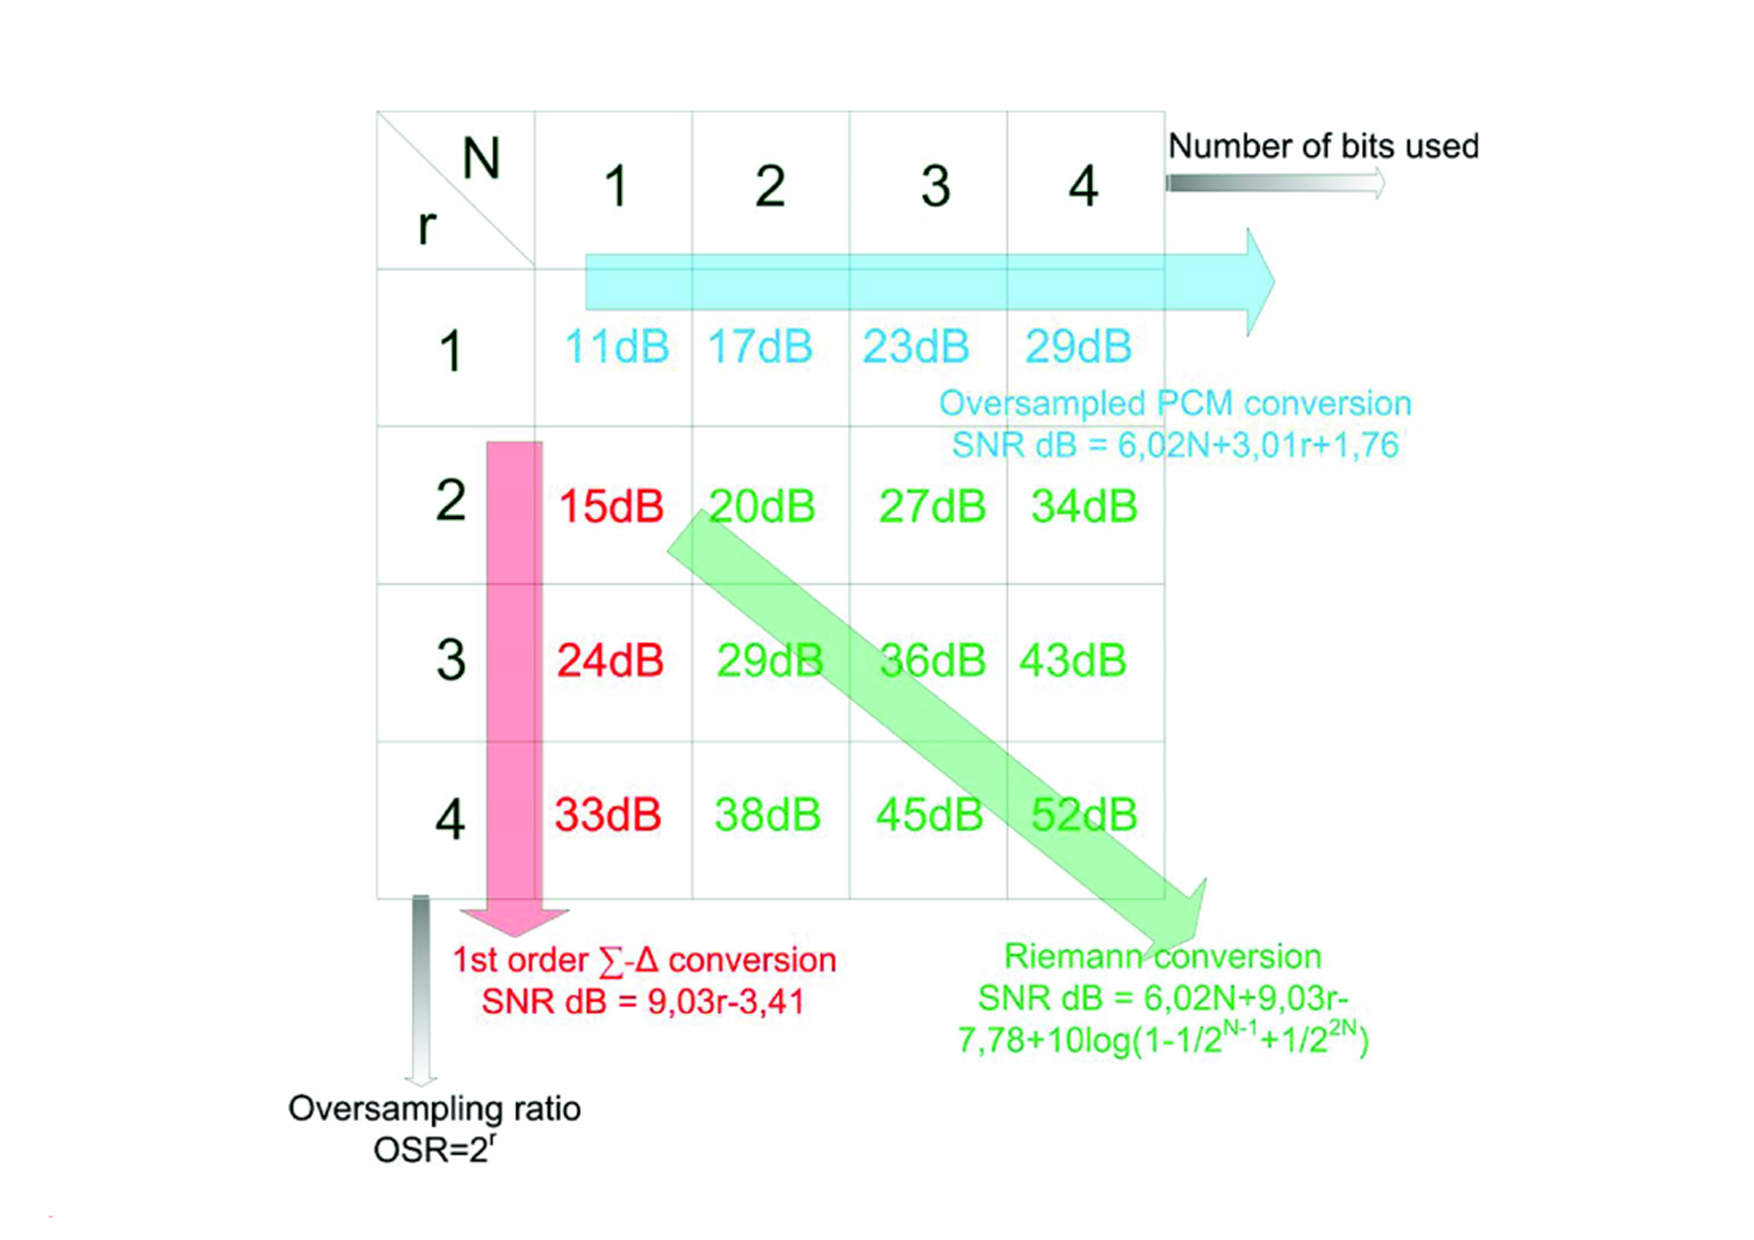
\includegraphics[width=\textwidth]{SQNR.pdf}
	\caption{Table of theoretically \gls{ab:sqnr} for a full scale sine wave over resolution and \gls{ab:osr} \cite{DevalRivetVeyrac2015}}
	\label{fig:TableSQNR}
\end{figure}

The table states the theoretical achievable \gls{ab:snr} with respect to these two parameters.
The parameter N describes the number of bits used for the resolution and r the binary logarithm of the \gls{ab:osr}, respectively.
Here the \gls{ab:osr} is defined as
\begin{equation}
OSR =  \frac{f_{sampling}}{2 f_{signal,max}} = 2^r,
\end{equation}
which leads to
\begin{equation}
f_{sampling} =  2^{r+1}*f_{signal,max}
\end{equation}
with respect to r.
As you can see in Figure \ref{fig:TableSQNR} the Riemann Conversion (green) performance is the best for a minimum number of bits and a \gls{ab:osr}, with respect to the parameter r, of two.
Performing a digital-to-analog conversion with one bit resolution, the $\Sigma - \Delta$ conversion fits the best.
For $ r = 1$ the \gls{ab:pcm} conversion yields the best \gls{ab:sqnr}.\\
In the Riemann Conversion it yields, that every increase in the number of bits will increase the \gls{ab:sqnr} by \SI{7}{\decibel}, while increasing the parameter r, will increase the \gls{ab:sqnr} by \SI{9}{\decibel} \cite{VeyracRivetDevalEtAl2016}.
Equation \ref{eq:SNR_RiemannPumpConversion}
\begin{equation}
	\text{SNR } [\si{\dB}] \approx 6.02N + 9.03r - 7.78 + 10\log_{10}(1 - \frac{1}{2}^{N-1} + \frac{1}{2}^{2N})
	\label{eq:SNR_RiemannPumpConversion}
\end{equation}
stated an approximation to calculate the theoretical achievable \gls{ab:snr} for a full scale sine wave with the Riemann Conversion \citep{DevalRivetVeyrac2015}.
For the sake of simplicity the formula \ref{eq:SNR_RiemannPumpConversion} was not derived in this context.
For further details see \cite{VeyracRivetDevalEtAl2014},\cite{VeyracRivetDevalEtAl2016} and \cite{Kester2009}.
%As stated in \cite{VeyracRivetDevalEtAl2014}, simulation results showed a \gls{ab:snr} of \SI{30}{\decibel} for $N = 3$ and $r = 2$, which exceeds the approximation of \SI{27}{\decibel}.

\section{Conclusion of the fundamentals}
In contrast to classical current steering topologies the Riemann Pump concept rather makes use of the derivative at sampling points than to sample the absolute value.
In order to reconstruct the analog signal, the digital code thus has to be integrated.

In this chapter the implementation of the Riemann Pump in a system design has been presented.
After the description of the classification and application, the concept of the custom \gls{ab:dac} has been described.
After explaining a simple charge pump, a multi bit resolution \gls{ab:dac} have been presented.
The designed custom \gls{ab:dac} has been compared to conventional \gls{ab:dac} concepts.
A concise evaluation states that the Riemann Pump is a great improvement for conventional digital-to-analog conversion concepts.
%The signal was generated by integrating a current over time which charged a capacitor.
% Therefore the Riemann Pump is a arbitrary waveform generator and also a high speed digital-to-analog converter
% a theoretical signal is processed with matlab
%This signal can consist of many different signals (different carriers and modulation types). 
%This signal is sampled with the given set of slopes. 
%The minimization of the error leads to the Riemann Code. 
%With this Riemann Code the driver circuit is controlled. This leads to an analog signal formed by the digital input signal. 